\section{Efficient Enumeration of Ladder Lotteries and its Application}

%%Intro
In the Efficient Enumeration of Ladder Lotteries and its Application, written by Matsui, Nakada, Nakano Uehara and Yamanaka,
the authors provide an algorithm for generating $OptL\{\pi\}$ 
for any $\pi$, in $\mathcal{O}(1)$ per ladder~\cite{A1}. The authors refer to this algorithm as {\sc FindAllChildren}
which can be found in Algorithm~\ref{Alg:FindAllChildren}. 
\begin{algorithm}[!htp]
	\begin{algorithmic}[1]
		\Function{FindAllChildren}{$ladder$, $cleanLevel$, $n$}
			\State $currentRoute \gets n$
			\While{$currentRoute \geq cleanLevel$}
				\State going top left to bottom right 
				\For{$bar \in currentRoute$}
					\State $row \gets$ row of $bar$ in $ladder$ 
					\State $col \gets$ col of $bar$ in $ladder$
					\State $lowerNeighbor \gets ladder[row-1][col]$
					\If{$lowerNeighbor$ is right swappable}
						\State {\sc RightSwap($ladder$, $bar$, $lowerNeighbor$)}
						\State {\sc {\sc FindAllChildren}($ladder$, $y+1$, $n$)}
						\State {\sc LeftSwap($ladder$, $bar$, $lowerNeighbor$)}
					\EndIf
				\EndFor
				\State $currentRoute \gets currentRoute-1$
			\EndWhile
			\State $currentRoute \gets cleanLevel-1$
			\For{$bar \in currentRoute$}
				\State $row \gets$ row of $bar$ in $ladder$ 
				\State $col \gets$ col of $bar$ in $ladder$
				\State $lowerNeighbor \gets ladder[row-1][col]$
				\If{$lowerNeighbor$ is right swappable \textbf{and} is the rightmost bar of $currentRoute-1$}
					\State {\sc RightSwap($ladder$, $bar$)}
					\State {\sc FindAllChildren($ladder$, $cleanLevel$, $n$)}
					\State {\sc LeftSwap($ladder$, $bar$)}
				\EndIf
			\EndFor
		\EndFunction
	\end{algorithmic}
	\caption{The algorithm for listing $OptL\{\pi\}$.}
	\label{Alg:FindAllChildren}
\end{algorithm}
\pagebreak

One will note that two helper functions, {\sc RightSwap} and {\sc LeftSwap}, are required to complete 
{\sc FindAllChildren}. The details of these algorithms are not found 
in the paper~\cite{A1}. Thus, these algorithms and their details can be found in the Appendix in Algorithm \ref{Alg:RightSwap}
and Algorithm \ref{Alg:LeftSwap}.
{\sc FindAllChildren} is the first algorithm for generating $OptL\{\pi\}$.\newline
{\sc FindAllChildren} enumerates $OptL\{\pi\}$ as a tree of ladders.

%%Put this in the Appendix

%%DONE PUT IN Appendix

%%%%%%%%%%%%%%%%%%%%%%%%%%%%%%%FIND ALL CHILDREN ALGORITHM%%%%%%%%%%%%%%%%%%%%%%%%%%%%%



%%%%%%%%%%%%%%%%%%END ALGORITHM%%%%%%%%%%%%%%%%%%%%%%%%%%



{\sc FindAllChildren} was used in this thesis to generate the sample data that aided in finding solutions for 
the Gray Code Problem in Chapter 3 and the Minimum Height Problem in Chapter 4.  
Therefore, this algorithm is paramount for the findings of this thesis. 
To see the tree structure generated by {\sc FindAllChildren} for $OptL\{(4,3,2,1)\}$ 
please refer to Figure~\ref{Fig:TreeFAC}. 
\begin{figure}[h]
	\centering 
	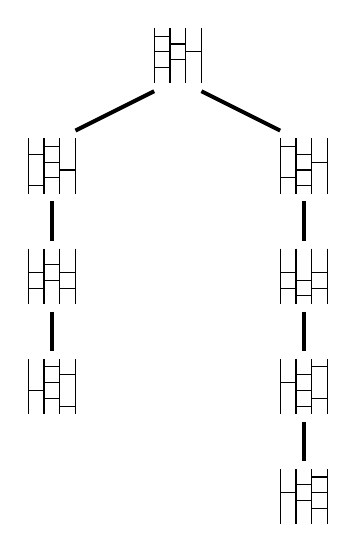
\begin{tikzpicture}
		%%L1
		\draw(5, 10) to (5, 9.3);
			\draw(5, 9.9) to (5.2, 9.9);
			\draw(5.2, 9.8) to (5.4, 9.8);
			\draw(5.4, 9.7) to (5.6, 9.7);
		\draw(5.2, 10) to (5.2, 9.3);
			\draw(5, 9.7) to (5.2, 9.7);
			\draw(5.2, 9.6) to (5.4, 9.6);
		\draw(5.4, 10) to (5.4, 9.3);
			\draw(5, 9.5) to (5.2, 9.5);
		\draw(5.6, 10) to (5.6, 9.3);
		%L2
		\draw[line width = .5mm](5, 9.2) to (4, 8.7);
		\draw[line width = .5mm](5.6, 9.2) to (6.6, 8.7);
			%%L2
			\draw(3.4, 8.6) to (3.4, 7.9);
				\draw(3.4, 8.4) to (3.6, 8.4);
				\draw(3.4, 8) to (3.6, 8);
			\draw(3.6, 8.6) to (3.6, 7.9);
				\draw(3.6, 8.5) to (3.8, 8.5);
				\draw(3.6, 8.3) to (3.8, 8.3);
				\draw(3.6, 8.1) to (3.8, 8.1);
			\draw(3.8, 8.6) to (3.8, 7.9);
				\draw(3.8, 8.2) to (4, 8.2);
			\draw(4.0, 8.6) to (4.0, 7.9);

				%%level
				\draw[line width = .5mm](3.7, 7.8) to (3.7, 7.3);
			\draw(3.4, 7.2) to (3.4, 6.5);
				\draw(3.4, 6.9) to (3.6, 6.9);
				\draw(3.4, 6.7) to (3.6, 6.7);
			\draw(3.6, 7.2) to (3.6, 6.5);
				\draw(3.6, 7) to (3.8, 7);
				\draw(3.6, 6.8) to (3.8, 6.8);
			\draw(3.8, 7.2) to (3.8, 6.5);
				\draw(3.8, 6.9) to (4, 6.9);
				\draw(3.8, 6.7) to (4, 6.7);
			\draw(4.0, 7.2) to (4.0, 6.5);

		%%L3
			\draw(6.6, 8.6) to (6.6, 7.9);
				\draw(6.6, 8.5) to (6.8, 8.5);
				\draw(6.8, 8.4) to (7, 8.4);
				\draw(7, 8.3) to (7.2, 8.3);
			\draw(6.8, 8.6) to (6.8, 7.9);
				\draw(6.8, 8.2) to (7, 8.2);
				\draw(6.8, 8) to (7, 8);
			\draw(7, 8.6) to (7, 7.9);
				\draw(6.6, 8.1) to (6.8, 8.1);
			\draw(7.2, 8.6) to (7.2, 7.9);
			
			
			\draw[line width = .5mm](6.9, 7.8) to (6.9, 7.3);

			\draw(6.6, 7.2) to (6.6, 6.5);
				\draw(6.6, 6.9) to (6.8, 6.9);
				\draw(6.6, 6.7) to (6.8, 6.7);
			\draw(6.8, 7.2) to (6.8, 6.5);
				\draw(6.8, 6.8) to (7, 6.8);
				\draw(6.8, 6.6) to (7, 6.6);
			\draw(7.0, 7.2) to (7.0, 6.5);
				\draw(7, 6.9) to (7.2, 6.9);
				\draw(7, 6.7) to (7.2, 6.7);
			\draw(7.2, 7.2) to (7.2, 6.5);

			\draw[line width = .5mm](3.7, 6.4) to (3.7, 5.9);

			\draw(3.4, 5.8) to (3.4, 5.1);
				\draw(3.4, 5.4) to (3.6, 5.4);
			\draw(3.6, 5.8) to (3.6, 5.1);
				\draw(3.6, 5.7) to (3.8, 5.7);

				\draw(3.6, 5.5) to (3.8, 5.5);
				\draw(3.6, 5.3) to (3.8, 5.3);
			\draw(3.8, 5.8) to (3.8, 5.1);
				\draw(3.8, 5.6) to (4, 5.6);
				\draw(3.8, 5.2) to (4, 5.2);
			\draw(4.0, 5.8) to (4.0, 5.1);

			\draw[line width = .5mm](6.9, 6.4) to (6.9, 5.9);

			
			\draw(6.6, 5.8) to (6.6, 5.1);
				\draw(6.6, 5.5) to (6.8, 5.5);
			\draw(6.8, 5.8) to (6.8, 5.1);
				\draw(6.8, 5.6) to (7, 5.6);

				\draw(6.8, 5.4) to (7, 5.4);
				\draw(6.8, 5.2) to (7, 5.2);
			\draw(7.0, 5.8) to (7.0, 5.1);
				\draw(7.0, 5.7) to (7.2, 5.7);
				\draw(7.0, 5.3) to (7.2, 5.3);
			\draw(7.2, 5.8) to (7.2, 5.1);

			\draw[line width = .5mm](6.9, 5) to (6.9, 4.5);

			\draw(6.6, 4.4) to (6.6, 3.7);
				\draw(6.6, 4.1) to (6.8, 4.1);
			\draw(6.8, 4.4) to (6.8, 3.7);
				\draw(6.8, 4.2) to (7, 4.2);

				\draw(6.8, 4) to (7, 4);
			\draw(7.0, 4.4) to (7.0, 3.7);
				\draw(7.0, 4.3) to (7.2, 4.3);
				\draw(7.0, 4.1) to (7.2, 4.1);
				\draw(7.0, 3.9) to (7.2, 3.9);
			\draw(7.2, 4.4) to (7.2, 3.7);



	\end{tikzpicture}
	\caption{The tree structure of $OptL\{(4,3,2,1)\}$ generated by {\sc FindAllChildren}}
	\label{Fig:TreeFAC}
\end{figure}
\pagebreak
{\sc FindAllChildren} is based on several key concepts. One of which is the local swap operation 
which has already been discussed. The next fundamental concept is the \emph{route} of an element, 
which is the sequence of bars the element travels along in order to reach its final position in the 
sorted permutation. The bars are read from top to bottom. For every bar, two elements cross 
the bar, therefore the bar is associated with the route of the greater of the two elements~\cite{A1}. 
In Figure~\ref{Fig:Route} the route of element $4$ is the sequence of bars 
$(4,1),(4,2),(5,4)$. To see the route of an element please refer to Figure~\ref{Fig:Route}. When a 
right swap operation occurs, the bar of the route associated with a lesser element is 
swapped above two bars of a route associated with a greater element. For example, in Figure~\ref{fig:rightSwap} in the right ladder, 
the bar $(3,1)$ which is associated with the route of element $3$ is right swapped above the two bars $(5,1)$ and $(5,3)$ 
both of which are associated with the route of $5$.\par 
\begin{figure}[h]
	\centering
	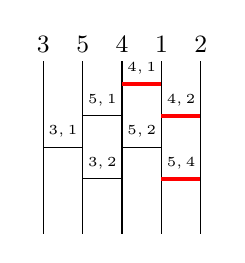
\begin{tikzpicture}
		\draw(0, 0) to (0, 2.2);
			\node at(.25, 1.3){\tiny{$3,1$}};
			\draw(0, 1.1) to (.5, 1.1);
		\draw(.5, 0) to (.5, 2.2);
			\node at(.75, 1.7){\tiny{$5,1$}};
			\draw(.5, 1.5) to (1, 1.5);
			\node at(.75, .9){\tiny{$3,2$}};
			\draw(.5, .7) to (1, .7);
		\draw(1, 0) to (1, 2.2);
			\node at(1.25, 2.1){\tiny{$4,1$}};
			\draw[line width=.5mm, red ](1, 1.9) to (1.5, 1.9);
			\node at(1.25, 1.3){\tiny{$5,2$}};
			\draw(1, 1.1) to(1.5, 1.1);
		\draw(1.5, 0) to (1.5, 2.2);
			\node at(1.75, 1.7){\tiny{$4,2$}};
			\draw[line width=.5mm, red ](1.5, 1.5) to (2, 1.5);
			\node at(1.75, .9){\tiny{$5,4$}};
			\draw[line width=.5mm, red ](1.5, .7) to (2, .7);
		\draw(2, 0) to (2, 2.2);


		\node at(0.0, 2.4){\small{$3$}};
		\node at(0.5, 2.4){\small{$5$}};
		\node at(1.0, 2.4){\small{$4$}};
		\node at(1.5, 2.4){\small{$1$}};
		\node at(2.0, 2.4){\small{$2$}};
	\end{tikzpicture}
	\caption{The route of element 4=(4,1),(4,2),(5,4).}
	\label{Fig:Route}
\end{figure}



The \emph{clean level} is defined as one more than the largest 
element associated with any bar that has undergone a right swap operation. 
For example, if the largest element associated with a bar that has undergone a 
right swap operation is element $4$, then the clean level is $5=4+1$.
 Please refer to Figure~\ref{Fig:CleanLevel} for an example of the clean level.
 If no bars have been right swapped, then the clean level is $1$.
If the largest element to have undergone a right swap operation is the maximal element in $\pi$, 
then the clean level is $max+1$.\pagebreak

\begin{figure}[t]
	\centering 
	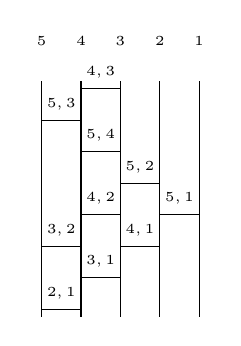
\begin{tikzpicture}
		\draw(0, 0) to (0, 3);
			\node at(.25, 2.7){\tiny{$5,3$}};
			\node at(.25, 1.1){\tiny{$3,2$}};
			\node at(.25, .3){\tiny{$2,1$}};
			\draw(0, 2.5) to (.5, 2.5);			
			\draw(0, .9) to (.5, .9);
			\draw(0, .1) to (.5, .1);

		\draw(.5, 0) to (.5, 3);
			\node at(.75, 3.1){\tiny{$4,3$}};
			\node at(.75, 2.3){\tiny{$5,4$}};
			\node at(.75, 1.5){\tiny{$4,2$}};
			\node at(.75, .7){\tiny{$3,1$}};

			\draw(.5, 2.9) to (1, 2.9);
			\draw(.5, 2.1) to (1, 2.1);
			\draw(.5, 1.3) to (1, 1.3);
			\draw(.5, .5) to (1, .5);
		\draw(1, 0) to (1, 3);
			\node at(1.25, 1.9){\tiny{$5,2$}};
			\node at(1.25, 1.1){\tiny{$4,1$}};

			\draw(1, 1.7) to (1.5, 1.7);
			\draw(1, .9) to (1.5, .9);
		\draw(1.5, 0) to (1.5, 3);
			\node at(1.75, 1.5){\tiny{$5,1$}};
			\draw(1.5, 1.3) to (2, 1.3);
		\draw(2, 0) to (2, 3);

		%%%%%%%%%%%%%%%%%%%%%%%%%%%%
		\node at(0, 3.5){\tiny{$5$}};
		\node at(.5, 3.5){\tiny{$4$}};
		\node at(1, 3.5){\tiny{$3$}};
		\node at(1.5, 3.5){\tiny{$2$}};
		\node at(2, 3.5){\tiny{$1$}};
\end{tikzpicture}
	\caption{A ladder with a clean level of $6$. The largest element whose associated bars have undergone a right swap operation is $5$}
	\label{Fig:CleanLevel}
\end{figure}


Each $OptL\{\pi\}$ has a unique ladder with a clean level of one. This ladder 
is known as the \emph{root ladder}. The root ladder is the root of the tree structure 
produced from {\sc FindAllChildren}. Unlike every other ladder in the tree, 
the root ladder cannot be derived from a local swap operation. Thus, the root ladder 
must be created by another algorithm other than {\sc FindAllChildren}. 
The authors do not provide details on how to create the root ladder. Thus, an 
algorithm for creating the root ladder can be found in the Appendix in Algorithm~\ref{Alg:RootLadder}.
The details of the root ladder are also explained in the Appendix.
Given all permutations of order $n$, the root ladder for the descending permutation requires 
the most rows. 
\begin{theorem}
  The number of rows required for the root ladder of the descending permutation is $2(n-1) - 1$.
\end{theorem}
\begin{proof}
  The number of rows for the ladder data-structure is calculated a follows: When a bar is added to the ladder it can be added 
  to an already existing row or to a new row. 
  If the current state of the ladder is empty then adding the first bar produces the second ladder in
  $L_{n}$. Since the bars are being added bottom right to top left, and the first bar to be added belongs 
  to the $nth$ route, then it must be added to $row=n-1$, $col=n-1$. As bars of the $nth$ route get 
  continuously added to the ladder, each bar is added a row above the previous bar and to a column 
  to the left of the column of the previous bar.
  Since no two bars of the $nth$ route can be on the same row, this will require $n-1$ rows. Note, if they were added to the same 
  row, then the left end point of the right bar would be touching the right end point of the left bar which is disallowed. Once the 
  bars of the $nth$ element are added, the bars of the $n-1th$ route will be added. The $n-1th's$ first bar 
  will be added to the $n-2$ column, otherwise it would be directly below the first bar of the $nth$ route, which is a violation. 
  Since the first bar of the $n-1$'s element is added to column $n-2$, then it must be given a new row, otherwise its right end point 
  will be touching  the left end point of the first bar of route $n$. The remaining $n-2$ bars of element $n-1$
  will be added bottom right to top left, but none of their end points will touch the end points of element $n$ seeing as they will 
  always be two columns apart from any bar in $n's$ route. The same logic applies to element $n-2$, it will require one extra row for its 
  first bar, in order not to touch the first bar of element $n-1$, but the remainder of its bars will always be two columns away from 
  the remainder of the bars for $n-1$, etc. Therefore there are $n-1$ rows required for the $nth$ element and each subsequent 
  element, $k$ requires only one new row. Since $2 \leq k < n$, then there are $(n-2)$ additional rows required for the ladder. Note that element 
  $1$ has no bars in its route. Therefore there are $(n-1)$ rows required for element $n's$ bars  plus $(n-2)$ rows required for 
  all the remaining $2 \leq k < n$ routes. In conclusion the number of rows required is $(n-1) + (n-2) = 2(n-1)-1$. 
  See figure for the tree of ladders 
  generated by {\sc ModifiedSJT} for $n=4$. Note that the maximum number of rows required is $2(n-1)-1=2(3)-1=5$.
\end{proof}



%%Root ladder subsection




%%DONE Appendix SECTION

In concluding the section on the enumeration problem, we have analyzed the original paper along with 
making additions to the algorithm {\sc FindAllChildren} by providing four essential algorithms 
for the completion of {\sc FindAllChildren}. The algorithms are Algorithm~\ref{Alg:RootLadder}, Algorithm~\ref{Alg:RightSwap},
Algorithm~\ref{Alg:LeftSwap} and Algorithm~\ref{Alg:ShiftSubLadder} which can be found in the Appendix. In concert, these five algorithms solve the enumeration 
problem which lists $OptL\{\pi\}$ in $O(1)$ time per ladder. 

